\documentclass{article}
\usepackage[utf8]{inputenc}
\usepackage{textcomp}
\usepackage{graphicx}
\usepackage{float}
\usepackage{array}
\usepackage{amsmath} % Math aligning equation
\usepackage{verbatim} % Command \verb
\usepackage{titlesec} % Righe di separazione
\usepackage{subcaption}
\usepackage[table]{xcolor}
\usepackage{tikz}
\usepackage{listings}

% Tabelle
\usepackage{tabu}
\usepackage{caption} 
\captionsetup[table]{skip=2pt}

% Impostazioni di pagina e margini
\usepackage[a4paper, margin=2.54cm]{geometry}

% Spacing nelle liste
\usepackage{enumitem}
\setlist{topsep=2pt, itemsep=3pt, partopsep=3pt, parsep=3pt}

% Cambio di nome di contenuti Latex
\renewcommand*\contentsname{Indice}
\renewcommand{\figurename}{Figura}
\renewcommand{\tablename}{Tabella}

% Checkmarks
\usepackage{pifont}
\newcommand{\cmark}{\ding{51}} % V
\newcommand{\xmark}{\ding{55}} % X

% Header & Footer
\usepackage{fancyhdr}
\pagestyle{fancy}
\fancyhf{}
\lhead{Prova finale di Reti Logiche - a.a. 2021/2022}
\rhead{Roberto Giandomenico}
\cfoot{\thepage}

% Titolo e informazioni
\title{Prova finale di Reti Logiche}
\author{Roberto Giandomenico}
\date{Anno Accademico 2021/2022}

\begin{document}

%==== Title Page
\thispagestyle{empty} 
\begin{titlepage}

    \begin{figure}[h]
        \vspace{5pt}
        \centering
        
\includegraphics[width=0.4\textwidth]{Resources/logo_polimi.png}
        \label{fig:logo_polimi}
        \vspace{5pt}
    \end{figure}

    \begin{center}
       \vspace*{5cm}
       {\huge Prova Finale (Progetto di Reti Logiche)}
       \vspace{1cm}
        \begin{large}   
        
            {Prof. Fabio Salice - Anno 2021/2022}
           \vspace{11cm}
            
            {Roberto Giandomenico (Codice Persona  - Matricola )}
           \vspace{2cm}
           
        \end{large}
   \end{center}
\end{titlepage}
\tableofcontents
\pagebreak



%%%%%%%%%%%%%%%%%%%%%%%%%%%%%%%%%%%%%%%
%%%%%%%%%%%% INTRODUZIONE %%%%%%%%%%%%%
%%%%%%%%%%%%%%%%%%%%%%%%%%%%%%%%%%%%%%%
\section{Introduzione} \label{subsection-introduz}

\subsection{Scopo del progetto}
Sia data una sequenza di parole da 8 bit ciascuna.\\
L’obiettivo del progetto è l’implementazione di un componente hardware descritto in VHDL che, letti i dati da memoria, sia in grado di applicarvi l’algoritmo di codifica convoluzionale con rapporto \(\frac{1}{2}\) ed infine restituisca il risultato scrivendolo in memoria.

\subsection{Descrizione generale}
La memoria da cui il componente legge e su cui scrive i dati è sincrona, a indirizzamento a byte e con uno spazio degli indirizzi a 16 bit. Il componente, servendosi della memoria, segue in ordine i seguenti passaggi:
\vspace{3.5pt}
\begin{enumerate}
    \item legge all'indirizzo di memoria \verb|0| il numero di parole da codificare;
    \item partendo dall'indirizzo \verb|1|, legge e serializza le parole ottenendo una sequenza di bit;
    \item su questa sequenza applica la codifica convoluzionale \(\frac{1}{2}\) raddoppiando, di fatto, il numero di bit;
    \item la nuova sequenza di bit viene infine scritta in memoria a partire dall'indirizzo \verb|1000|.
\end{enumerate}
\vspace{5pt}
Questa procedura viene ripetuta per tutte le parole presenti. Il numero massimo di parole da dover codificare è 255.\\
Inoltre il componente deve funzionare correttamente con un periodo di clock di almeno \verb|100 ns|.

\subsection{Codifica convoluzionale}
Il codificatore convoluzionale con tasso di trasmissione \(\frac{1}{2}\) è un componente che per ogni bit che riceve in ingresso genera la sua codifica in 2 bit. Si può rappresentare come una macchina a stati di Mealy con un bit per l’ingresso e 2 bit per l’uscita come in Figura \ref{fig:Cod_Conv}.

\begin{figure}[h]
    \vspace{15pt}
    \centering
    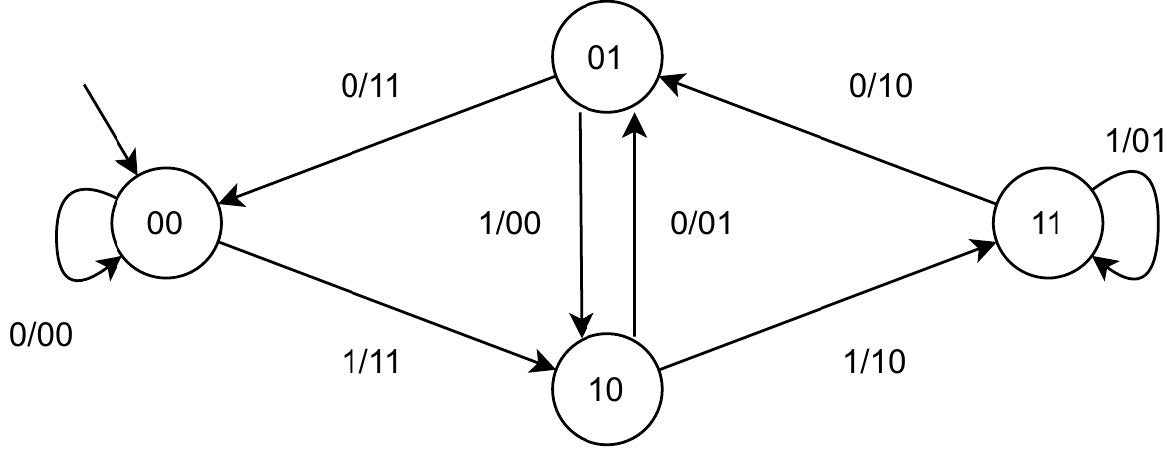
\includegraphics[width=0.8\textwidth]{Resources/Cod_Conv.jpg}
    \caption{Codifica convoluzionale con rapporto \(\frac{1}{2}\)}
    \label{fig:Cod_Conv}
    \vspace{5pt}
\end{figure}
\pagebreak

\subsection{Dati e memoria}
Il componente deve leggere da una memoria con indirizzamento al byte. Si assume come prerequisito che il contenuto della memoria non verrà modificato durante l'esecuzione. La quantità di parole \verb|W| da codificare è memorizzata all'indirizzo \verb|0|. Il primo byte della sequenza è memorizzato all'indirizzo \verb|1|. Lo stream di parole in uscita, invece, deve essere memorizzato a partire dall'indirizzo \verb|1000|.\\
Si legge da una cella della RAM scrivendo l’indirizzo in \verb|o_address| e abilitandone la lettura, cioè ponendo \verb|o_en|=1 e \verb|o_we|=0. \\
Si scrive in una cella della RAM scrivendo l’indirizzo in \verb|o_address| e abilitandola in scrittura, cioè ponendo \verb|o_en|=1 e \verb|o_we|=1. \\
Come si può notare dalla Figura \ref{fig:Memoria_RAM}, l’ultimo indirizzo utilizzato della memoria è $1000 + 2 \times (W-1) + 1$ che, dato $W_{max}$ = 255 da specifica, può valere al massimo 1509.

\begin{figure}[h]
    \vspace{10pt}
    \centering
    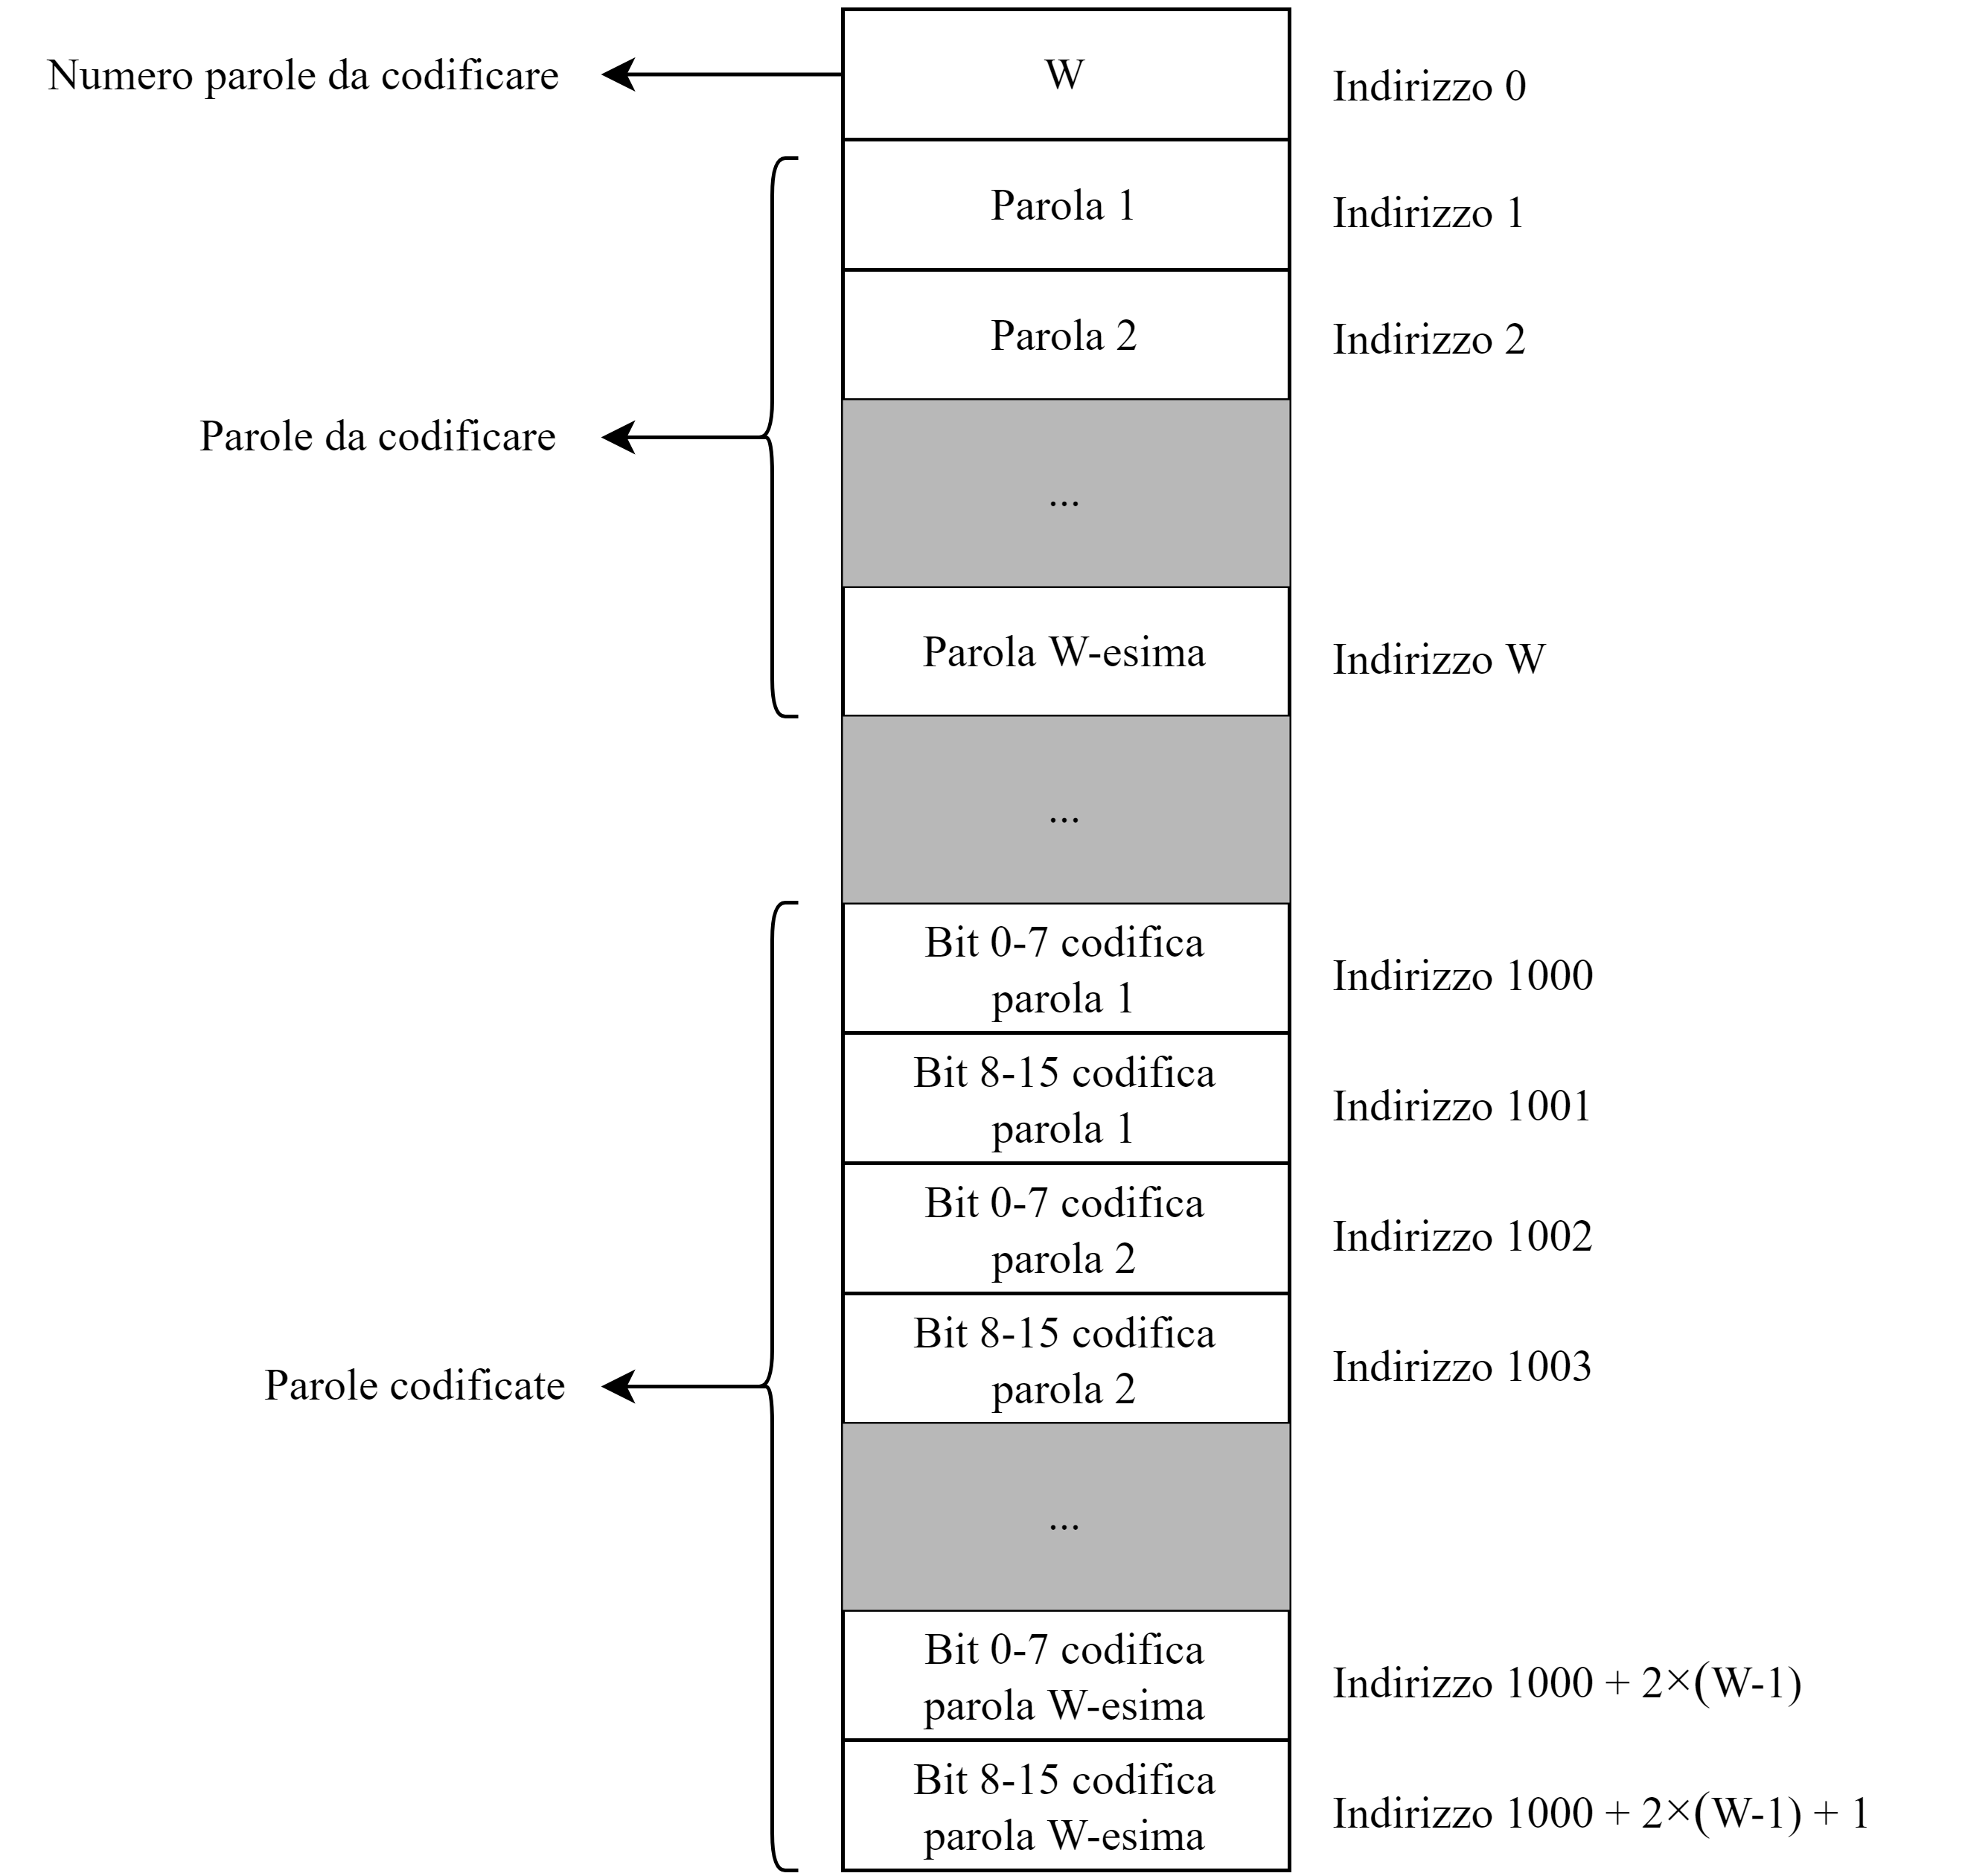
\includegraphics[width=0.9\textwidth]{Resources/Memoria.png}
    \caption{Indirizzi della RAM rilevanti}
    \label{fig:Memoria_RAM}
    \vspace{5pt}
\end{figure}

\subsection{Esempio}
Il componente legge dalla memoria (Tabella \ref{tab:Mem_Lett}) all’indirizzo \verb|0| il numero di parole totale da codificare. Successivamente partendo dall’indirizzo \verb|1| legge la prima parola, la quale viene serializzata e il singolo bit viene dato in ingresso al codificatore convoluzionale come in Tabella \ref{tab:Conv}. Quest’ultimo produce due bit in ogni istante \verb|t|, i quali vengono scritti in memoria a partire dall’indirizzo \verb|1000|.
Una volta codificata la prima parola il codificatore continua con le successive fino ad averle codificate tutte.\\
Il contenuto della memoria alla fine della codifica è riportato in Tabella \ref{tab:Mem_Scrit}.

\begin{table}[ht]
    \begin{minipage}{0.45\textwidth}
        \centering
        \begin{tabular}{||c|c||}
            \hline
            Indirizzo & Contenuto \\
            \hline
            \verb|0| & \verb|00000010| \\ 
            \verb|1| & \verb|10100010| \\ 
            \verb|2| & \verb|01001011| \\ 
            \hline
        \end{tabular}
        \vspace{5pt}
        \caption{Contenuto iniziale memoria}
        \label{tab:Mem_Lett}
    \end{minipage}
    \hfill
    \begin{minipage}{0.45\textwidth}
        \centering
        \begin{tabular}{||c|c||}
            \hline
            Indirizzo & Contenuto \\
            \hline
            \verb|1001| & \verb|11010001| \\ 
            \verb|1002| & \verb|11001101| \\ 
            \verb|1003| & \verb|11110111| \\ 
            \verb|1004| & \verb|11010010| \\ 
            \hline
        \end{tabular}
        \vspace{5pt}
        \caption{Contenuto finale memoria}
        \label{tab:Mem_Scrit}
    \end{minipage}
\end{table}

\begin{table}[h]
    \centering
    \begin{tabular}{||c|c c c c c c c c||}
        \hline
        \verb|t|   & 0 & 1 & 2 & 3 & 4 & 5 & 6 & 7 \\
        \hline
        \verb|Uk|  & 1 & 0 & 1 & 0 & 0 & 0 & 1 & 0 \\
        \verb|P1k| & 1 & 0 & 0 & 0 & 1 & 0 & 1 & 0 \\
        \verb|P2k| & 1 & 1 & 0 & 1 & 1 & 0 & 1 & 1 \\
        \hline
        \hline
        \verb|t|   & 8 & 9 & 10 & 11 & 12 & 13 & 14 & 15 \\
        \hline
        \verb|Uk|  & 0 & 1 &  0 &  0 &  1 &  0 &  1 &  1 \\
        \verb|P1k| & 1 & 1 &  0 &  1 &  1 &  0 &  0 &  1 \\
        \verb|P2k| & 1 & 1 &  1 &  1 &  1 &  1 &  0 &  0 \\
        \hline
    \end{tabular}
    \vspace{5pt}
    \caption{Codifica convoluzionale al tempo t}
    \label{tab:Conv}
\end{table}

\subsection{Interfaccia del componente}
Il componente descritto presenta la seguente interfaccia:
\begin{lstlisting}[basicstyle=\small, language=VHDL]
entity project_reti_logiche is
port (
	i_clk       : in std_logic;
	i_rst       : in std_logic;
	i_start     : in std_logic;
	i_data      : in std_logic_vector(7 downto 0);
	o_address   : out std_logic_vector(15 downto 0);
	o_done      : out std_logic;
	o_en        : out std_logic;
	o_we        : out std_logic;
	o_data      : out std_logic_vector(7 downto 0)
);
end project_reti_logiche;
\end{lstlisting}
\vspace{10pt}

In particolare:
\vspace{3.5pt}
\begin{itemize}
    \item \verb|i_clk| è il segnale di \verb|CLOCK| in ingresso generato dal Test Bench;
    \item \verb|i_rst| è il segnale di \verb|RESET| invocato sempre all'inizio della computazione e talvolta durante la codifica;
    \item \verb|i_start| è il segnale di \verb|START| che fa partire il processo di codifica;
    \item \verb|i_data| è il vettore a 8 bit tramite cui è possibile leggere il dato da memoria;
    \item \verb|o_address| è il vettore in uscita che serve ad indicare l'indirizzo di memoria desiderato;
    \item \verb|o_done| è il segnale di notifica che comunica la fine dell’elaborazione di tutte le parole in uscita;
    \item \verb|o_en| è il segnale di \verb|ENABLE| che, quando posto ad \verb|1|, permette di comunicare con la memoria;
    \item \verb|o_we| è il segnale di \verb|WRITE ENABLE| che, quando posto ad \verb|1|, permette la scrittura in memoria; deve essere \verb|0| in caso di sola lettura;
    \item \verb|o_data| è il vettore contenente la stringa da salvare in memoria.
\end{itemize}
\vspace{10pt}
L’elaborazione inizia quando viene alzato il segnale \verb|i_start| e termina quando il componente alza il segnale \verb|o_done|. Solo successivamente il segnale \verb|i_start| dovrà essere abbassato.





%%%%%%%%%%%%%%%%%%%%%%%%%%%%%%%%%%%%%%%
%%%%%%%%%%%% ARCHITETTURA %%%%%%%%%%%%%
%%%%%%%%%%%%%%%%%%%%%%%%%%%%%%%%%%%%%%%
\newpage
\section{Architettura}
Per la progettazione del componente è stata scelta l'implementazione tramite una macchina a stati finiti (FSM) di Mealy non completamente specificata. Infatti il valore delle uscite è funzione degli ingressi e per alcune transizioni è indifferente.

\subsection{Macchina a stati}
La macchina implementata (Figura \ref{fig:FSM}) è composta dai seguenti 13 stati principali.

\subsubsection{\texttt{IDLE} state}
Stato iniziale e di default della macchina, in cui si attende il segnale di \verb|i_start| e in cui si torna in caso di ricezione di un segnale di \verb|reset|.

\subsubsection{\texttt{W\_SAVE} state}
Stato in cui si legge e si salva il numero di parole da codificare, presente all'indirizzo \verb|0|. Nel caso questo numero sia nullo, si alza il segnale \verb|o_done|. In caso contrario si può salvare \verb|W| nel registro ausiliario \verb|words_num|.

\subsubsection{\texttt{WORD\_READ\_SETUP} state}
Stato in cui si pongono \verb|o_en|=1 e \verb|o_we|=0. L'array \verb|o_address| sarà l'indirizzo della parola che si vuole leggere.

\subsubsection{\texttt{WORD\_READ} state}
In questo stato si effettua la lettura della parola e la si salva nel registro \verb|loaded_word|.

\subsubsection{\texttt{ENCODER\_STATE} state}
Questo stato segue il codificatore convoluzionale durante il suo percorso e può assumere il valore di uno dei quattro sotto-stati \verb|S00|, \verb|S01|, \verb|S10| o \verb|S11|. In input riceve il bit specifico della parola da codificare.

\subsubsection{\texttt{RECORD\_ENCODED\_BIT} state}
Stato in cui si aggiorna il registro da 16 bit contenente le due parole finali con i due bit appena ricevuti in output dal codificatore convoluzionale.

\subsubsection{\texttt{UPDATE\_BIT\_COUNTER} state}
Stato in cui si aggiorna il numero di bit già letti e processati della singola parola.

\subsubsection{\texttt{CHECK\_WORD\_END} state}
Si controlla quanti bit sono stati letti e codificati. Non appena si è completata la lettura dei primi 4 bit, si è pronti per scrivere la prima parola in memoria (codificata in 8 bit). Se sono stati letti tutti gli 8 bit dell'attuale parola presa in input si è, di fatto, conclusa la codifica ed è possibile registrare anche la seconda parte della parola in memoria.

\subsubsection{\texttt{WRITE\_WORD\_1} state}
Stato in cui si pongono \verb|o_en|=1 e \verb|o_we|=1 in modo da poter registrare in memoria i primi 8 bit della codifica, cioè la prima parola in output all'indirizzo $1000 + 2 \times words\_counter$.

\subsubsection{\texttt{WRITE\_WORD\_2} state}
Stato in cui si pongono \verb|o_en|=1 e \verb|o_we|=1 in modo da poter registrare in memoria i successivi 8 bit della codifica, cioè la seconda parola in output all'indirizzo $1000 + 2 \times words\_counter + 1$.

\subsubsection{\texttt{UPDATE\_COUNTER} state}
Si incrementa il contatore delle parole lette fino a questo momento in attesa di un nuovo confronto con il totale numero di parole da leggere.

\subsubsection{\texttt{CHECK\_END} state}
Si verifica se tutte le parole sono già state codificate. In caso affermativo si pone \verb|o_done|=1. In caso contrario si continua con la codifica delle successive parole.

\subsubsection{\texttt{DONE} state}
Stato per la terminazione di un’istanza di computazione ponendo il segnale \verb|o_done|=1. Riporta allo stato di \verb|IDLE| non appena riceve il segnale \verb|i_start|=0.

\begin{figure}[h]
    \vspace{10pt}
    \centering
    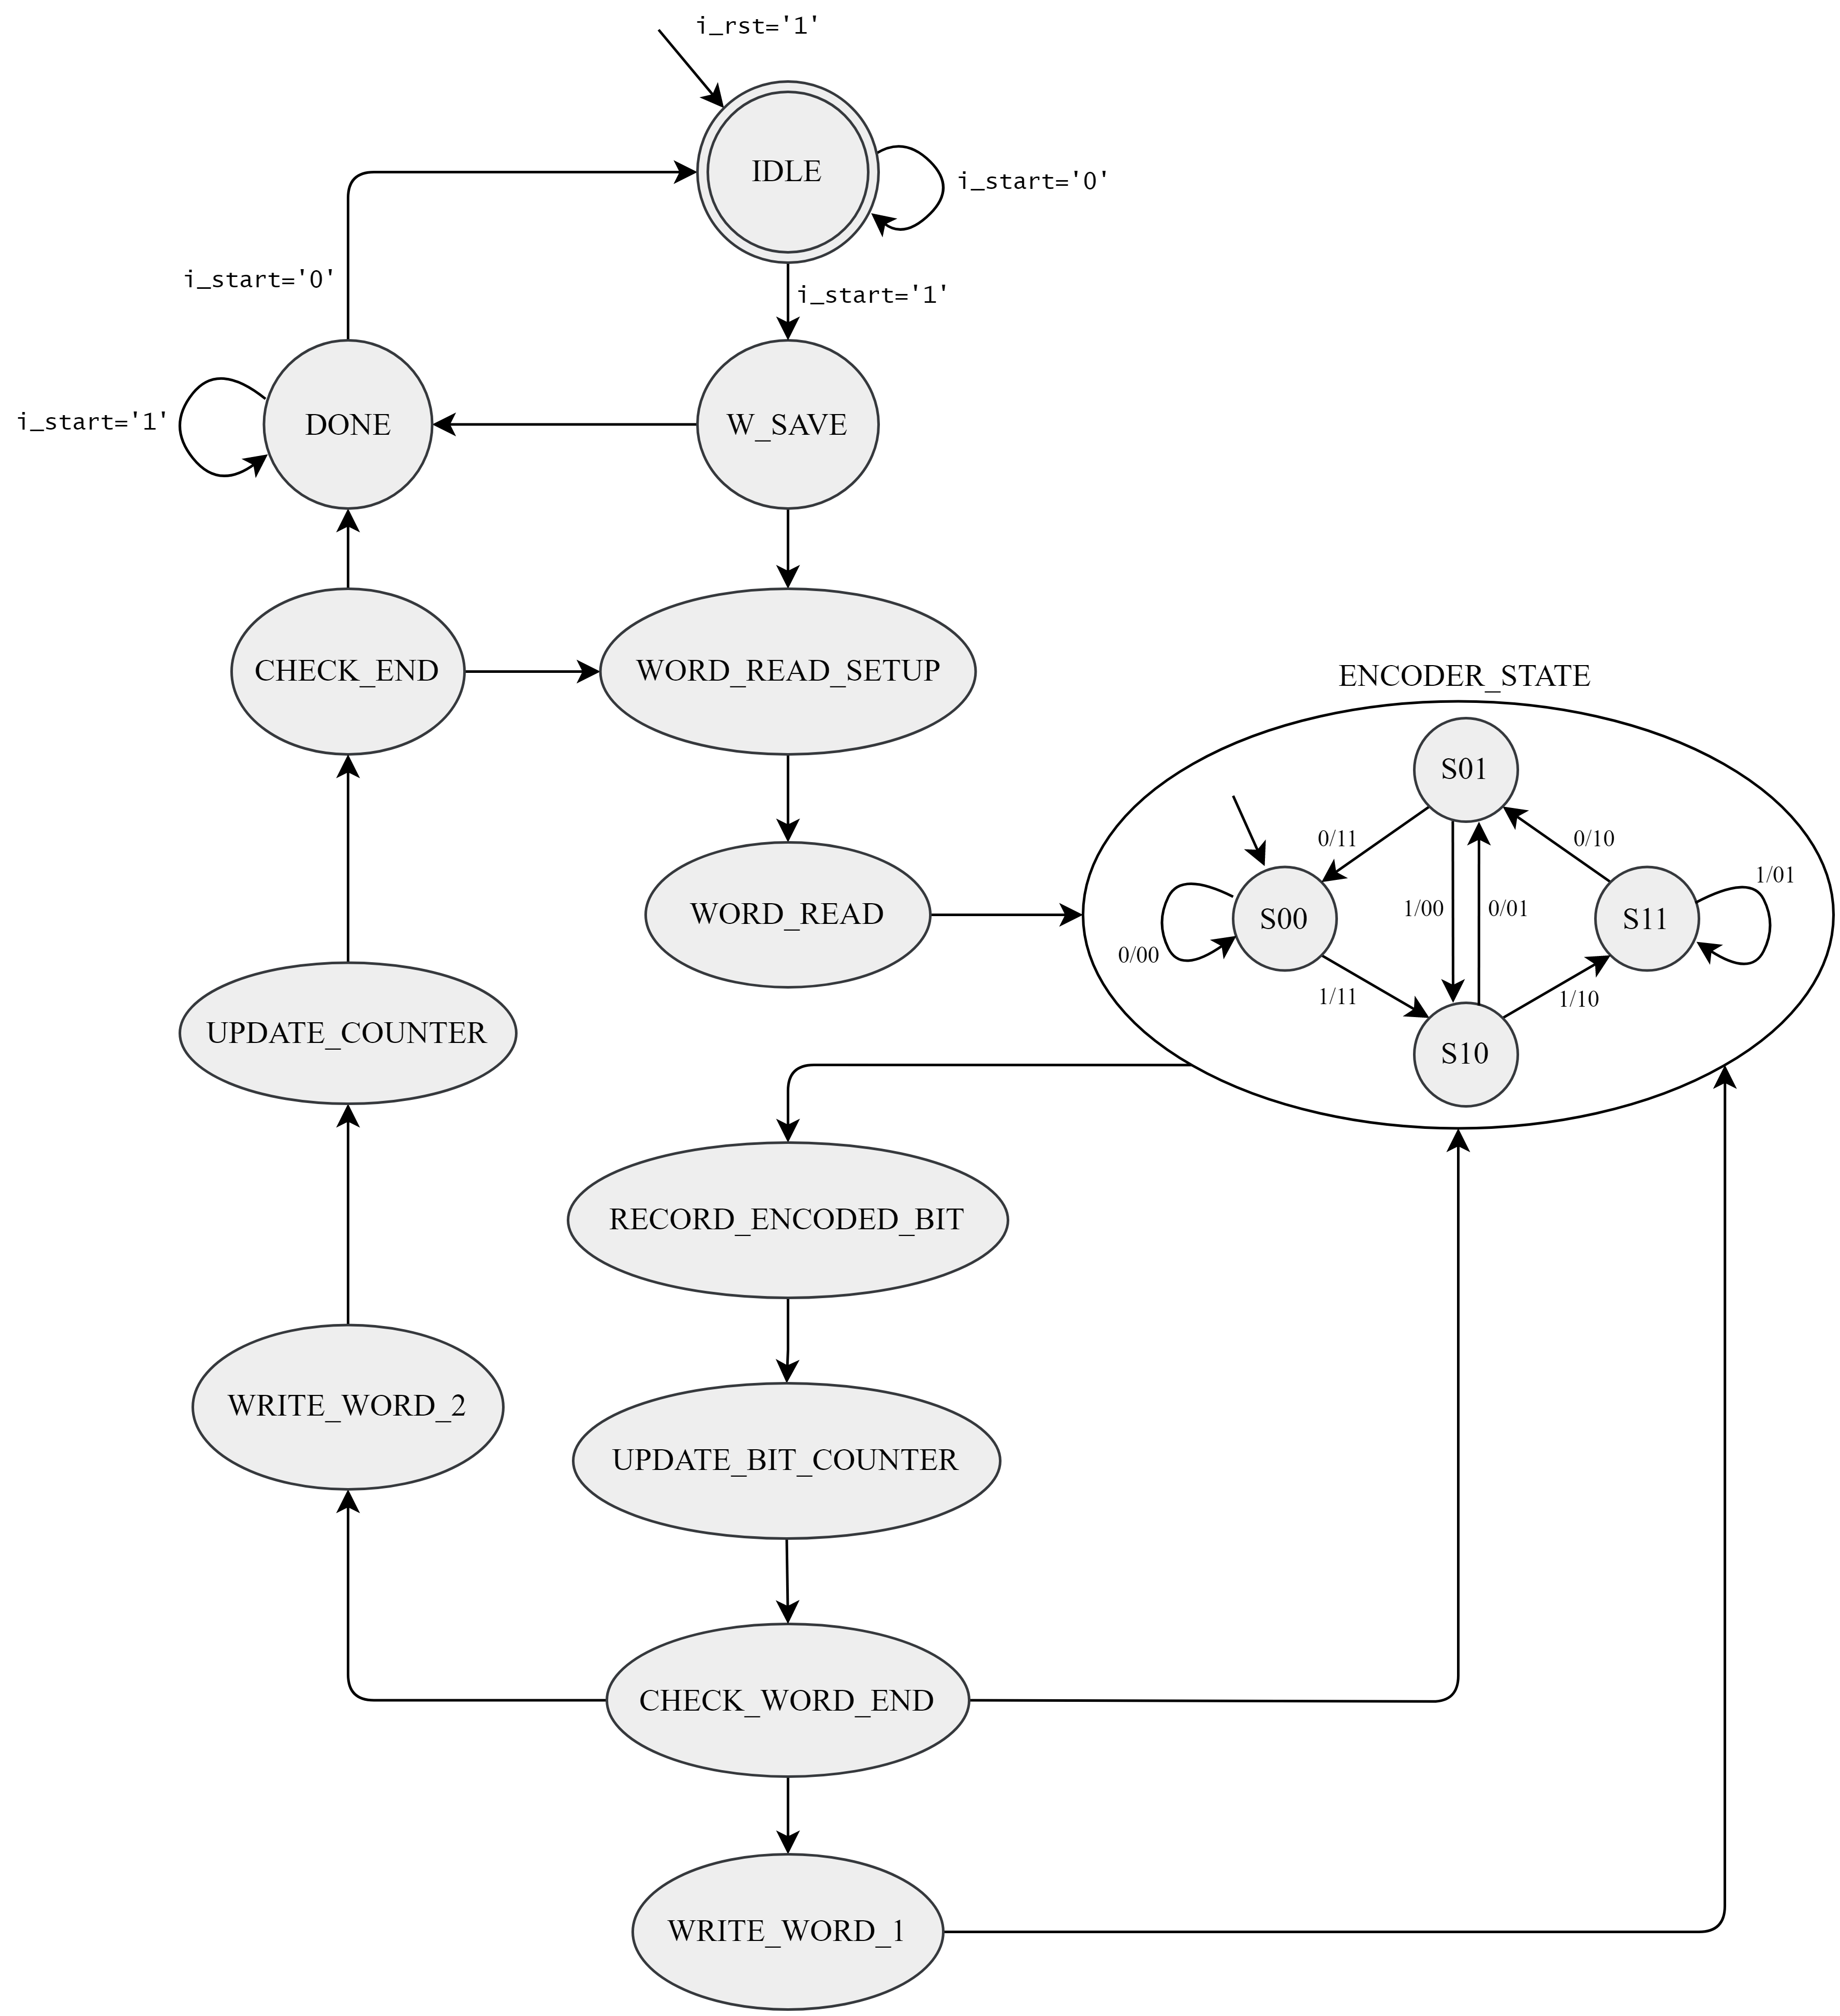
\includegraphics[width=0.9\textwidth]{Resources/FSM.png}
    \vspace{2pt}
    \caption{Macchina a stati finiti}
    \label{fig:FSM}
\end{figure}

\newpage
\subsection{Variables e signals}
Sono qui riportati i signals utilizzati come ausilio per l'elaborazione dei dati.
\vspace{3.5pt}
\begin{itemize}
    \item \verb|words_num|: registro in cui si salva il valore di \verb|W| dopo la sua lettura;
    \item \verb|words_counter|: registro in cui si salva il numero delle parole lette e codificate fino a quel momento;
    \item \verb|loaded_word|: registro in cui viene salvata la parola letta dalla memoria RAM e da codificare;
    \item \verb|word_bit_counter|: registro che conta il numero bit già codificati della parola in input;
    \item \verb|encoder_state|: memorizza l'ultimo stato visitato del codificatore convoluzionale;
    \item \verb|encoder_output|: registro in cui si salva l'output su 2 bit del codificatore;
    \item \verb|encoded_word|: registro in cui si salva, durante il processo di codifica, l'intera parola codificata su 16 bit.
\end{itemize}





%%%%%%%%%%%%%%%%%%%%%%%%%%%%%%%%%%%%%%%
%%%%%%%%%%%%%% SINTESI %%%%%%%%%%%%%%%%
%%%%%%%%%%%%%%%%%%%%%%%%%%%%%%%%%%%%%%%
\newpage
\section{Sintesi}

\subsection{Tool e FPGA}
La sintesi e l’implementazione sono state fatte usando il software \textit{VIVADO 2016.4}. La FPGA target utilizzata è la Artix-7 FPGA xc7a200tfbg484-1.

\subsection{Report di utilizzo}
Effettuando la sintesi risulta il seguente utilizzo:
\begin{center}
    \verb=+-------------------------+------+-------+------------+-----------+-------+=
    \verb=|        Site Type        | Used | Fixed | Prohibited | Available | Util% |=
    \verb=+-------------------------+------+-------+------------+-----------+-------+=
    \verb=| Slice LUTs*             |   94 |     0 |          0 |    134600 |  0.07 |=
    \verb=|   LUT as Logic          |   94 |     0 |          0 |    134600 |  0.07 |=
    \verb=|   LUT as Memory         |    0 |     0 |          0 |     46200 |  0.00 |=
    \verb=| Slice Registers         |   86 |     0 |          0 |    269200 |  0.03 |=
    \verb=|   Register as Flip Flop |   86 |     0 |          0 |    269200 |  0.03 |=
    \verb=|   Register as Latch     |    0 |     0 |          0 |    269200 |  0.00 |=
    \verb=| F7 Muxes                |    0 |     0 |          0 |     67300 |  0.00 |=
    \verb=| F8 Muxes                |    0 |     0 |          0 |     33650 |  0.00 |=
    \verb=+-------------------------+------+-------+------------+-----------+-------+=
\end{center}
Come si può notare dal report sull'utilizzo, il codice VHDL è stato scritto in modo da evitare l’inferenza di latch, con il preciso scopo di rendere l’intero componente sincronizzato sul fronte di salita del clock. Sono stati così evitati gli effetti di propagazioni indesiderate dei segnali. \\
Tutte le percentuali di utilizzo risultano essere molto minori del 100\%, dunque il modulo implementato occupa solo una piccola parte della FPGA.

\subsection{Report di timing}
Dal report si ottiene:
\begin{center}
    \verb|Slack (MET) :     96.283ns  (required time - arrival time)              |\\
\end{center}
\\
Analizzando il report sul timing possiamo notare che il \textit{Worst Negative Slack (WNS)} è di \verb|96.283ns|, il quale sta ad indicare che il componente potrebbe funzionare correttamente anche con periodi di clock molto più bassi. In particolare, il componente è in grado di funzionare ad una frequenza di clock \textit{$f_{clk}$} maggiore di quella data da specifica che è pari a \(\frac{1}{100ns}\) = 10 MHz. Più precisamente, il minimo periodo utilizzabile risulta:
\begin{center}
    \textit{T_{min} = T_{clk} - WNS = 100ns - 96.283ns = 3.717ns}\\
\end{center}
\\
e quindi si ottiene la massima frequenza di funzionamento:
\begin{center}
    \textit{f_{max} = \(\frac{1}{T_{min}}\) = \(\frac{1}{3.717ns}\) \approx 269.03MHz}\\
\end{center}






%%%%%%%%%%%%%%%%%%%%%%%%%%%%%%%%%%%%%%%
%%%%%%%%%%%%%% TESTING %%%%%%%%%%%%%%%%
%%%%%%%%%%%%%%%%%%%%%%%%%%%%%%%%%%%%%%%
\newpage
\section{Testing del componente}
Allo scopo di verificare il corretto funzionamento del componente sintetizzato, il codice è stato testato dapprima con i Test Bench forniti insieme alle specifiche e in seguito con test costruiti ad hoc aventi i seguenti obiettivi:
\vspace{3.5pt}
\begin{enumerate}
    \item verificare i casi limite;
    \item verificare il corretto funzionamento dei segnali;
    \item verificare la solidità del componente.
\end{enumerate}
\vspace{3.5pt}

\subsection{Test e casi limite}
Le modalità di simulazione eseguite sono due: \textit{Behavioural} e \textit{Post-Synthesis Functional}. Di seguito sono riportati i casi di test più significativi.

\subsubsection{Sequenza minima}
Nel caso della sequenza minima viene scritto zero all'indirizzo \verb|0|. In questo modo il componente, come in Figura \ref{fig:Seq_Min}, dopo aver letto che il numero di parole da elaborare è zero, alza il segnale \verb|o_done| e termina la codifica.\\
\begin{figure}[h]
    \vspace{5pt}
    \centering
    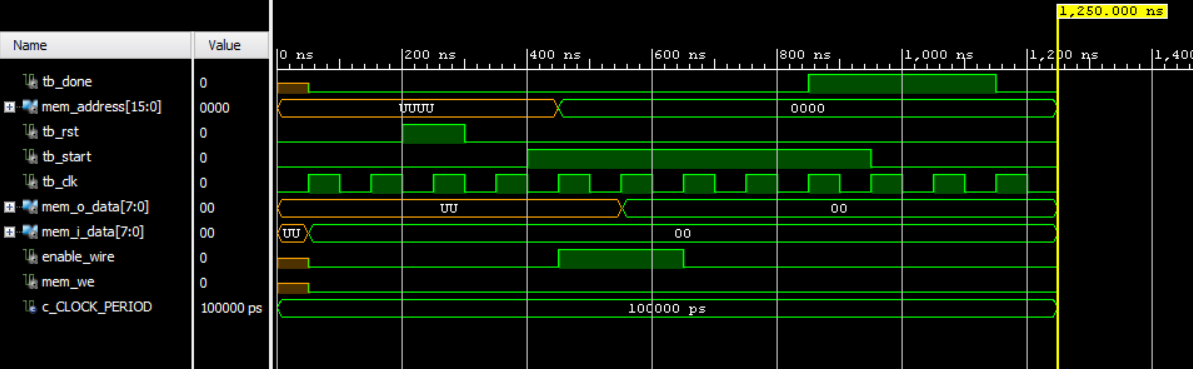
\includegraphics[width=\textwidth]{Resources/Seq_Min.png}
    \caption{Simulazione sequenza minima}
    \label{fig:Seq_Min}
    \vspace{5pt}
\end{figure}

\subsubsection{Sequenza massima}
Nel caso di sequenza massima viene inserito 255 all'indirizzo \verb|0|. Come mostrato in Figura \ref{fig:Seq_Max}, il componente riesce a codificare tutte le parole compresa l'ultima.\\
\begin{figure}[h]
    \vspace{5pt}
    \centering
    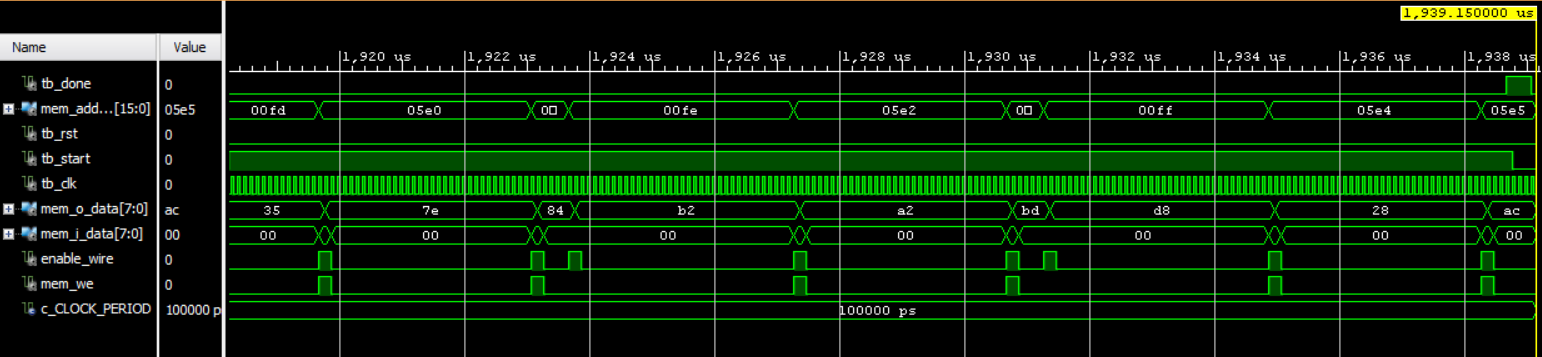
\includegraphics[width=\textwidth]{Resources/Seq_Max.png}
    \caption{Estratto simulazione sequenza massima}
    \label{fig:Seq_Max}
    \vspace{5pt}
\end{figure}

\subsubsection{Reset asincrono}
Il componente riceve durante la codifica un segnale di \verb|reset| e, come in Figura \ref{fig:Reset}, riesce a ricominciare la codifica correttamente dopo aver ricevuto un nuovo segnale di \verb|start|.\\
\begin{figure}[h]
    \vspace{5pt}
    \centering
    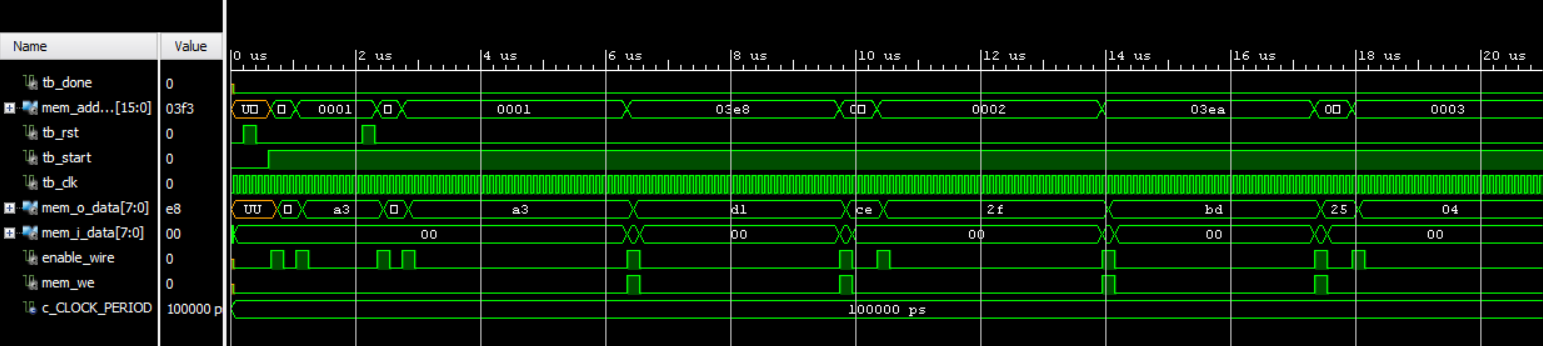
\includegraphics[width=\textwidth]{Resources/Reset.png}
    \caption{Estratto simulazione reset}
    \label{fig:Reset}
    \vspace{5pt}
\end{figure}

\subsubsection{Codifica continua}
Viene testata la capacità del componente di codificare più sequenze una dopo l'altra senza ricevere un segnale di \verb|reset|. Il componente, una volta terminata una sequenza, riesce ad iniziare correttamente la codifica di un nuovo flusso dopo aver ricevuto un nuovo segnale di \verb|start|. Un estratto è mostrato in Figura \ref{fig:Tre_Res}.
\begin{figure}[h]
    \vspace{5pt}
    \centering
    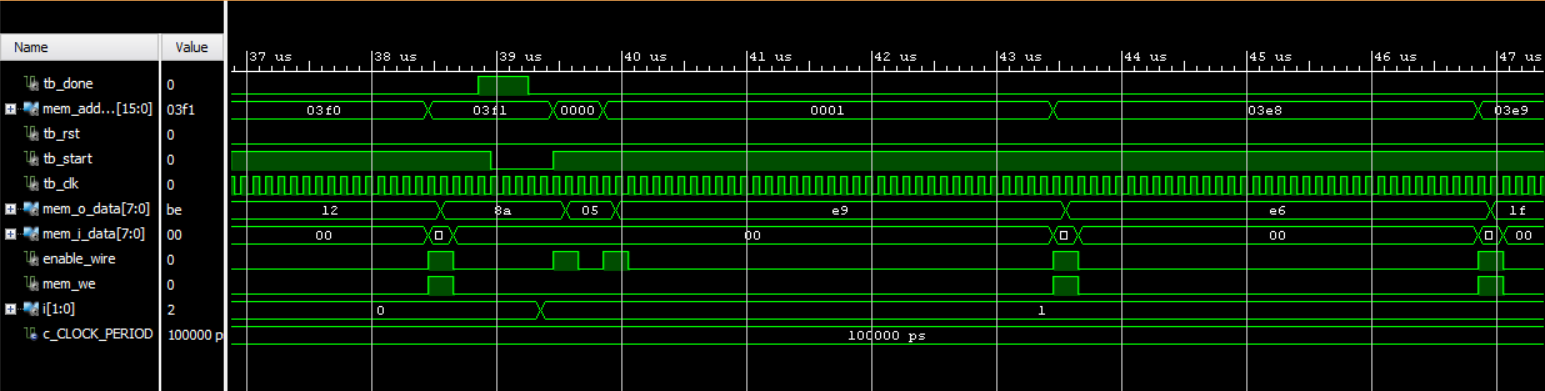
\includegraphics[width=\textwidth]{Resources/Tre_Res.png}
    \caption{Estratto simulazione di codifica continua}
    \label{fig:Tre_Res}
    \vspace{5pt}
\end{figure}

\subsubsection{Test Casuali}
Per aumentare la probabilità di trovare eventuali errori, il componente è stato sottoposto a numerosi Test Bench casuali generati utilizzando un applicativo scritto in Python.\\
La correttezza di tali simulazioni è stata poi verificata tramite la lettura del file di log.
\vspace{20pt}

\subsection{Osservazioni}
Il componente supera correttamente tutti i test proposti in precedenza sia a livello \textit{Behavioral} che \textit{Post-Synthesis}. Quest’ultimo tipo di simulazione è stato essenziale per verificare che eventuali ottimizzazioni applicate dal tool in fase di sintesi non influenzino il corretto funzionamento del componente.






%%%%%%%%%%%%%%%%%%%%%%%%%%%%%%%%%%%%%%%
%%%%%%%%%%%% CONCLUSIONE %%%%%%%%%%%%%%
%%%%%%%%%%%%%%%%%%%%%%%%%%%%%%%%%%%%%%%
\newpage
\section{Conclusione}
Il componente descritto nelle specifiche è stato sintetizzato con successo e tutte le simulazioni effettuate terminano con esito positivo.\\
La trasformazione della specifica in una macchina a stati finiti ha semplificato notevolmente la fase di architettura del modulo. Inoltre l'architettura è stata pensata per diminuire il più possibile l'overhead alla codifica utilizzando il minimo numero di stati possibili e minimizzando l'utilizzo di risorse, abbattendo così i tempi d’esecuzione del modulo e l'area occupata.\\
Dal punto di vista del design, si è scelto di utilizzare un'unica FSM senza componenti esterni, racchiudendo tutto in un solo processo.\\
Infine è possibile notare che il componente è in grado di funzionare ad una frequenza di clock molto più alta, all'incirca di 269.03 MHz.

\end{document}